



\section{Additional results}
In the following, we report extra results and observations on the performance of the proposed methods. In particular, we show how the Generalized Contrastive Loss function contributes to learn representations that better characterize the relevant parts of the input images for a robust computation of their similarity. Furthermore, we presents insights about how the GCL function contributes to a better regularization of the learned latent space.

\revised{We studied the effect of a different pooling layer by training our models on the MSLS dataset using a Global Average Pooling layer and report the results that we obtained.  
Furthermore, we evaluate our MSLS models on the Pittsburgh250k~\cite{Torii-PAMI2015} and TokyoTM~\cite{Torii-PAMI2015} benchmarks, and provide detailed results for the Extended CMU Seasons~\cite{sattler2018benchmarking} and RobotCar Seasons V2 datasets~\cite{sattler2018benchmarking}, divided by environment and weather condition. 
We also provide a comparison with the work of Thoma et al~\cite{thoma2020soft} on the CMU Seasons dataset. 
}

We study the effect that different threshold values for the ground truth similarity associated to the images have on the performance of our models. We consider two ground truth thresholds: one based on the GPS distance in meters between the locations in which images were taken, and another based on the annotated degree of similarity, $\psi$. 
 \revised{Finally, we provide extended results on the 7Scenes dataset, including the precision recall curves and a small test to evaluate our descriptors in a visual localization pipeline.}

\begin{figure}[!b]
    \centering
\subfloat[ResNet50-GeM-CL]{
\label{fig:tsneCL}
\includegraphics[width=.45\columnwidth]{figures/appendix/tsne/resnet50-GeM-CL-nowhitening-tsne-cph.jpg}}~\subfloat[ResNet50-GeM-GCL]{
\label{fig:tsneGCL}
\includegraphics[width=.45\columnwidth]{figures/appendix/tsne/resnet50-GeM-GCL-nowhitening-tsne-cph.jpg}}
    \caption{Visualization of the learned embedded space. We selected 1000 random positive pairs and 1000 random negative pairs from the MSLS Copenhagen set, computed the differences between their representations and projected them into a 2D space using T-SNE.}
    \label{fig:tsne}
\end{figure}

\subsection{Learned latent space }

In Fig.~\ref{fig:tsne}, we show the 2D projection of the vectors representing the difference of the latent space representation of 2000 image pairs (1000 positive and 1000 negative) randomly selected from the Copenhagen set of the MSLS dataset. For each pair, we compute the difference between the map and the query image latent representation. We use this as input to the t-SNE algorithm~\cite{tsne}, which projects the representations onto a 2D space. We visualize the vectors produced by two models with a ResNet50-GeM backbone, one trained using the CL function (Fig.~\ref{fig:tsneCL}) and the other using the GCL (Fig.~\ref{fig:tsneGCL}) function. The effect of the proposed GCL function is evident in the better regularized latent space, where the representation of similar image pairs (blue dots) are more consistently distributed towards the center of the space. The representations learned using the CL function, instead, form a more scattered and noisy distribution.


\begin{figure*}[!t]
    \centering
    %\includegraphics[width=\textwidth]{figures/appendix/activations.eps}
    {\fontsize{8pt}{11pt}
    \def\svgwidth{\textwidth}
      \input{figures/appendix/activations.pdf_tex}}
    \caption{CNN activations for the ResNet50-GeM and the VGG16-GeM models with CL and GCL for several input image pairs. The first two pairs, corresponding to the first four columns, are part of the MSLS test set. The third and fourth belong to the Pittsburgh30k and Tokyo 24/7 test set, respectively. We show the activations for the last layer of the backbone overlapped with the input images.}
    \label{fig:activations}
\end{figure*}








\begin{table*}[t!]
\centering
\caption{Ablation study on the considered datasets: all the models are trained on the MSLS train set and deploy a global average pooling layer. CL stands for Contrastive Loss and while GCL for our Generalized Contrastive Loss. For the cases in which PCA whitening is applied we report the dimensionality that achieves the best results on the MSLS validation set.}
\label{tab:ablation-avg}
\resizebox{\textwidth}{!}{%
\setlength\tabcolsep{1.5pt}
\begin{tabular}
{@{}lcccccccccccccccccccc@{}}
\toprule
\textbf{} & \textbf{} & \textbf{} & \multicolumn{3}{c}{\textbf{MSLS-Val}} & \multicolumn{3}{c}{\textbf{MSLS-Test}} & \multicolumn{3}{c}{\textbf{Pittsburgh30k}} & \multicolumn{3}{c}{\textbf{Tokyo24/7}} & \multicolumn{3}{c}{\textbf{RobotCar Seasons V2}} & \multicolumn{3}{l}{\textbf{Extended CMU Seasons}} \\
\textbf{Method} & \textbf{PCA$_w$} & \textbf{Dim} & \textbf{R@1} & \textbf{R@5} & \textbf{R@10} & \textbf{R@1} & \textbf{R@5} & \textbf{R@10} & \textbf{R@1} & \textbf{R@5} & \textbf{R@10} & \textbf{R@1} & \textbf{R@5} & \textbf{R@10} & \textbf{0.25m/2$\degree$} & \textbf{0.5m/5$\degree$} & \textbf{5.0m/10$\degree$} & \textbf{0.25m/2$\degree$} & \textbf{0.5m/5$\degree$} & \textbf{5.0m/10$\degree$} \\ \midrule
VGG-avg-CL & No & 512 & 28.8 & 47.0 & 53.9 & 16.9 & 30.5 & 36.4 & 28.9 & 53.7 & 64.8 & 10.5 & 24.1 & 35.6 & 1.0 & 6.4 & 34.4 & 0.9 & 3.0 & 22.7 \\
VGG-avg-GCL & No & 512 & 48.8 & 67.8 & 73.1 & 21.5 & 31.4 & 37.9 & 42.1 & 66.9 & 77.3 & 20.0 & 42.5 & 52.1 & 2.3 & 12.5 & 51.7 & 2.3 & 7.2 & 43.3 \\
VGG-avg-CL & Yes & 128 & 35.0 & 53.4 & 60.1 & 35.2 & 47.3 & 54.1 & 47.1 & 69.5 & 78.3 & 16.2 & 28.9 & 40.0 & 2.3 & 10.0 & 42.0 & 2.1 & 6.6 & 34.9 \\
VGG-avg-GCL & Yes & 256 & 54.5 & 72.6 & 78.2 & 32.9 & 49.0 & 56.5 & 56.2 & 76.7 & 83.9 & 28.6 & 45.7 & 54.9 & 3.6 & 15.3 & 57.1 & 3.7 & 11.2 & 52.5 \\ \midrule
ResNet50-avg-CL & No & 2048 & 44.3 & 60.3 & 65.9 & 24.9 & 39.0 & 44.6 & 54.0 & 75.7 & 83.1 & 20.6 & 40.0 & 50.2 & 3.1 & 12.6 & 51.0 & 2.6 & 7.8 & 43.4 \\
ResNet50-avg-GCL & No & 2048 & 59.6 & 72.3 & 76.2 & 35.8 & 52.0 & 59.0 & 62.5 & 82.7 & 88.4 & 24.1 & 44.1 & 54.6 & 2.9 & 12.9 & 56.3 & 3.1 & 9.7 & 55.1 \\
ResNet50-avg-CL & Yes & 2048 & 58.8 & 71.4 & 75.8 & 33.1 & 46.5 & 53.3 & 65.8 & 82.6 & 88.2 & 48.6 & 63.2 & 70.5 & 5.9 & 22.8 & 62.7 & 4.7 & 13.8 & 50.8 \\
ResNet50-avg-GCL & Yes & 1024 & 69.5 & 81.2 & 85.5 & 44.2 & 57.8 & 63.4 & 73.3 & 87.1 & 91.2 & 52.1 & 68.9 & 72.7 & 5.9 & 23.1 & 69.6 & 5.4 & 16.2 & 66.5 \\ \midrule
ResNet152-avg-CL & No & 2048 & 53.1 & 70.1 & 75.4 & 29.7 & 44.2 & 51.3 & 59.7 & 80.3 & 87.0 & 27.0 & 48.6 & 58.4 & 2.5 & 13.1 & 56.6 & 3.0 & 9.2 & 49.9 \\
ResNet152-avg-GCL & No & 2048 & 65.1 & 80.0 & 83.8 & 43.5 & 59.2 & 65.2 & 69.3 & 87.2 & 91.3 & 32.1 & 52.1 & 62.2 & 3.3 & 13.5 & 59.9 & 3.6 & 11.0 & 61.2 \\
ResNet152-avg-CL & Yes & 1024 & 63.0 & 77.7 & 81.5 & 37.7 & 51.6 & 56.9 & 68.8 & 85.9 & 90.4 & 49.8 & 67.3 & 74.3 & 5.4 & 22.2 & 64.8 & 4.8 & 14.3 & 59.9 \\
ResNet152-avg-GCL & Yes & 2048 & 75.8 & 87.4 & 89.7 & 52.7 & 68.1 & 74.2 & \textbf{77.9} & \textbf{90.4} & \textbf{93.5} & \textbf{64.4} & \textbf{77.8} & \textbf{83.2} & \textbf{6.2} & \textbf{23.9} & 70.0 & \textbf{5.7} & \textbf{17.0} & 66.5 \\ \midrule
ResNeXt-avg-CL & No & 2048 & 58.9 & 75.1 & 79.9 & 34.5 & 50.1 & 57.7 & 51.3 & 73.6 & 81.9 & 24.8 & 47.3 & 56.8 & 2.7 & 10.9 & 61.0 & 2.0 & 6.1 & 40.0 \\
ResNeXt-avg-GCL & No & 2048 & 72.2 & 85.1 & 87.3 & 51.5 & 66.9 & 71.7 & 62.9 & 81.0 & 87.1 & 39.4 & 58.1 & 68.9 & 2.7 & 12.4 & 63.1 & 3.3 & 10.2 & 57.7 \\
ResNeXt-avg-CL & Yes & 1024 & 71.6 & 84.7 & 88.0 & 46.5 & 62.9 & 68.9 & 69.2 & 85.3 & 89.6 & 44.8 & 63.5 & 73.6 & 4.8 & 20.4 & \textbf{70.6} & 4.6 & 13.4 & 58.6 \\
ResNeXt-avg-GCL & Yes & 1024 & \textbf{79.3} & \textbf{89.2} & \textbf{90.3} & \textbf{57.8} & \textbf{72.3} & \textbf{77.1} & 74.8 & 88.2 & 91.8 & 53.0 & 76.2 & 80.6 & 2.7 & 10.9 & 61.0 & 5.6 & 16.6 & \textbf{70.7} \\ \bottomrule

\end{tabular}%
}
\end{table*}




















\subsection{Network activation}

In Fig.~\ref{fig:activations}, we show the activation maps of the last convolutional layer of our models with a \revised{VGG16-GeM and a} ResNet50-GeM backbone, both trained using the Contrastive Loss function (CL) and the proposed Generalized Contrastive Loss (GCL) function.  We selected two example image pairs from the MSLS test set~\cite{msls} corresponding to the cities of Kampala and Stockholm, one from the Pittsburgh30k test set~\cite{Arandjelovic2017}, and one from the Tokyo 24/7 dataset~\cite{Torii-CVPR2013}. For all cases, we observed that the model trained with the GCL function produces higher activation for the common visual features of the images, and lower for the irrelevant parts (i.e. the road or the sky), in contrast to the model trained with the binary CL, which focuses less in the concerned areas of the pictures. In the example from Stockholm we can observe that our model does not respond to the cars (which vary from picture to picture), while it does respond strongly to the cranes (which are a more permanent feature). The example from Tokyo 24/7 is also particularly interesting: our model trained with the GCL function has high responses on the common parts of the images even under big changes of illumination. \revised{We observed that ResNet architectures tend to produce a peak of activation on the top left corner of the images. This does not seem to occur with the VGG architecture, so our intuition is that this artifact is due to the residuals. }


\revised{\subsection{Results with Global Average Pooling}
In addition to using GeM, we also trained the considered backbones (i.e. VGG16, ResNet50, ResNet152 and ResNeXt) using a Global Average Pooling on the MSLS dataset. We show the results in Table~\ref{tab:ablation-avg}. We observed that our method can reach good results with an even simpler pooling layer as is a Global Average Pooling, although a GeM layer usually leads to better results (see main paper). Our methods reaches good results on the validation and test sets of MSLS and generalizes well to unseen datasets such as Pittsburgh30k~\cite{Arandjelovic2017}, Tokyo24/7~\cite{Arandjelovic2017}, RobotCar Seasons V2~\cite{sattler2018benchmarking} and Extended CMU Seasons~\cite{sattler2018benchmarking}. As we observed also with the GeM models, the Global Average Pooling models can reach better performance when PCA whitening is applied, up to a 72.3\% top-5 recall on the test set of MSLS.
}






\begin{table}[t!]
\centering
\caption{Generalization results of the models trained on the MSLS dataset for the Pittsburgh250k and TokyoTM benchmarks.}
\label{tab:ablation-pitts250k}
\resizebox{\columnwidth}{!}{%
\begin{tabular}{@{}lcccccccc@{}}
\toprule
\textbf{} & \textbf{} & \textbf{} & \multicolumn{3}{c}{\textbf{Pittsburgh250k}} & \multicolumn{3}{c}{\textbf{TokyoTM}} \\ 
\textbf{Method} & \textbf{PCA$_w$} & \textbf{Dim} & \textbf{R@1} & \textbf{R@5} & \textbf{R@10} & \textbf{R@1} & \textbf{R@5} & \textbf{R@10} \\\midrule
 VGG-avg-CL & No & 512 & 20.2 & 38.0 & 47.2 & 38.9 & 58.5 & 67.2 \\
VGG-avg-GCL & No & 512 & 32.1 & 53.4 & 62.7 & 65.6 & 80.8 & 85.2 \\
VGG-avg-CL & Yes & 128 & 39.3 & 58.9 & 67.4 & 66.0 & 80.3 & 85.0 \\
VGG-avg-GCL & Yes & 256 & 51.3 & 71.0 & 78.0 & 78.6 & 87.7 & 90.8 \\
VGG-GeM-CL & No & 512 & 44.5 & 63.1 & 70.1 & 67.7 & 80.8 & 85.0 \\
VGG-GeM-GCL & No & 512 & 53.3 & 72.4 & 79.2 & 75.5 & 85.4 & 88.6 \\
VGG-GeM-CL & Yes & 512 & 65.1 & 81.2 & 85.8 & 83.7 & 91.1 & 93.3 \\
VGG-GeM-GCL & Yes & 512 & 73.4 & 86.4 & 89.9 & 88.2 & 93.2 & 94.7 \\\midrule
ResNet50-avg-CL & No & 2048 & 45.1 & 65.8 & 73.6 & 69.7 & 83.0 & 87.5 \\
ResNet50-avg-GCL & No & 2048 & 56.2 & 77.1 & 83.8 & 72.3 & 84.8 & 88.4 \\
ResNet50-avg-CL & Yes & 2048 & 70.6 & 85.4 & 89.5 & 90.5 & 94.8 & 96.0 \\
ResNet50-avg-GCL & Yes & 1024 & 74.6 & 87.9 & 91.6 & 91.7 & 95.7 & 96.8 \\
ResNet50-GeM-CL & No & 2048 & 54.8 & 74.2 & 80.7 & 73.3 & 85.4 & 89.2 \\
ResNet50-GeM-GCL & No & 2048 & 68.2 & 84.6 & 89.2 & 80.1 & 88.8 & 91.6 \\
ResNet50-GeM-CL & Yes & 1024 & 72.4 & 86.6 & 90.4 & 88.7 & 93.9 & 95.4 \\
ResNet50-GeM-GCL & Yes & 1024 & 80.9 & 91.4 & 94.3 & 92.2 & 95.6 & 96.8 \\\midrule
ResNet152-avg-CL & No & 2048 & 51.3 & 73.0 & 80.1 & 73.5 & 86.4 & 89.9 \\
ResNet152-avg-GCL & No & 2048 & 64.0 & 83.6 & 89.2 & 78.9 & 89.0 & 91.9 \\
ResNet152-avg-CL & Yes & 1024 & 69.6 & 85.9 & 90.6 & 90.7 & 95.1 & 96.3 \\
ResNet152-avg-GCL & Yes & 2048 & 80.9 & 92.2 & 95.3 & \textbf{94.0} & \textbf{96.7} & \textbf{97.3} \\
ResNet152-GeM-CL & No & 2048 & 60.7 & 79.0 & 85.1 & 77.8 & 88.3 & 91.2 \\
ResNet152-GeM-GCL & No & 2048 & 68.0 & 84.9 & 89.8 & 81.5 & 90.3 & 92.8 \\
ResNet152-GeM-CL & Yes & 2048 & 76.2 & 89.9 & 93.4 & 91.1 & 95.3 & 96.4 \\
ResNet152-GeM-GCL & Yes & 2048 & \textbf{83.8} & \textbf{93.7} & \textbf{96.1} & 93.1 & 96.1 & 96.8 \\\midrule
ResNeXt-avg-CL & No & 2048 & 44.2 & 65.8 & 73.9 & 69.0 & 82.3 & 86.3 \\
ResNeXt-avg-GCL & No & 2048 & 57.9 & 76.1 & 82.6 & 77.7 & 86.9 & 89.7 \\
ResNeXt-avg-CL & Yes & 1024 & 69.6 & 85.4 & 89.8 & 88.9 & 94.1 & 95.6 \\
ResNeXt-avg-GCL & Yes & 1024 & 74.7 & 88.0 & 91.7 & 89.6 & 94.6 & 95.9 \\
ResNeXt-GeM-CL & No & 2048 & 50.2 & 70.8 & 78.8 & 66.1 & 78.5 & 82.7 \\
ResNeXt-GeM-GCL & No & 2048 & 58.6 & 76.2 & 81.8 & 78.7 & 87.1 & 90.1 \\
ResNeXt-GeM-CL & Yes & 1024 & 70.3 & 85.2 & 89.6 & 87.2 & 93.1 & 94.5 \\
ResNeXt-GeM-GCL & Yes & 1024 & 78.2 & 90.1 & 93.1 & 91.8 & 95.4 & 96.6 \\ \bottomrule
\end{tabular}%
}
\end{table}





\revised{\subsection{Results on Pittsburgh250k and TokyoTM}
We evaluated the generalization of our models trained on MSLS to the Pittsburgh250k~\cite{Torii-PAMI2015} and TokyoTM~\cite{Arandjelovic2017} datasets. The test set of the former consists of 83k map and 8k query images taken over the span of several years in Pittsburgh, Pennsylvania, USA. The TokyoTM dataset consists of images collected using the Time Machine tool on Google Street View in Tokyo over several years. Its validation set is divided into a map and a query set, with 49k and 7k images.

The results that we obtained are in line with those reported in the main paper. Our models trained with a GCL function consistently generalize better to unseen datasets than their counterpart trained with a binary Contrastive Loss function. Their performance is further boosted if PCA whitening is applied, up to a top-5 recall of 93.7\% on Pittsburgh250k and 96.7\% on TokyoTM. }


\begin{table}[t!]
\centering
\caption{Detailed results on the Extended CMU dataset. The symbol $^\star$ denotes the models for which PCA whitening has been applied. }
\label{tab:cmu_detailed}
\resizebox{\columnwidth}{!}{%
\setlength\tabcolsep{1.5pt}
\begin{tabular}{@{}lcccc@{}}
\toprule
\textbf{} & \textbf{Mean} & \textbf{Urban} & \textbf{Suburban} & \textbf{Park} \\ 
\textbf{Method} & \textbf{\begin{tabular}[c]{@{}c@{}}0.25/0.5/10m \\ 2/5/10$\degree$\end{tabular}} & \textbf{\begin{tabular}[c]{@{}c@{}}0.25/0.5/10m \\ 2/5/10$\degree$\end{tabular}} & \textbf{\begin{tabular}[c]{@{}c@{}}0.25/0.5/10m \\ 2/5/10$\degree$\end{tabular}} & \textbf{\begin{tabular}[c]{@{}c@{}}0.25/0.5/10m \\ 2/5/10$\degree$\end{tabular}} \\\midrule
NetVLAD-64-Pitts30k & 5.3 / 15.9 / 66.3 & 10.7 / 27.8 / 84.1 & 2.9 / 11.2 / 63.5 & 2.4 / 8.9 / 50.1 \\
NetVLAD-64-Pitts30k$^\star$ & 5.8 / 17.6 / 70.3 & 11.6 / 30.3 / 87.5 & 3.3 / 12.5 / 68 & 2.7 / 10.2 / 54.2 \\
NetVLAD-64-MSLS & 1.3 / 4.5 / 31.9 & 2.9 / 8.4 / 49.6 & 0.8 / 3.4 / 29.7 & 0.3 / 1.6 / 15.2 \\
NetVLAD-64-MSLS$^\star$ & 3.9 / 12.1 / 58.4 & 7.6 / 20.3 / 77.2 & 2.6 / 9.7 / 58.9 & 1.6 / 6.3 / 37.0 \\
NetVLAD-16-MSLS & 1.7 / 5.5 / 39.1 & 3.7 / 10.0 / 57.3 & 1.1 / 4.5 / 38.6 & 0.4 / 1.9 / 19.8 \\
NetVLAD-16-MSLS$^\star$ & 4.4 / 13.7 / 61.4 & 8.4 / 22.1 / 76.9 & 3.0 / 11.4 / 63.1 & 1.9 / 7.4 / 41.9 \\
AP-GeM$^\star$ & 4.9 / 14.7 / 65.2 & 9.8 / 25.2 / 82.6 & 2.8 / 10.9 / 65.3 & 2.1 / 8 / 45.9 \\
NetVLAD-SARE$^\star$ & \textbf{6.4} / \textbf{19.4} / \textbf{75.5} & \textbf{12.5} / \textbf{32.4 }/ \textbf{90.7} & \textbf{3.9} / \textbf{14.7 }/ \textbf{76.3} & 3.0 / 11.3 / 57.6 \\\midrule
VGG-avg-CL & 0.9 / 3.0 / 22.7 & 2.0 / 5.8 / 39.4 & 0.6 / 2.3 / 21 & 0.2 / 0.7 / 6.5 \\
VGG-avg-GCL & 2.3 / 7.2 / 43.3 & 4.7 / 13.0 / 64.3 & 1.6 / 5.8 / 43.4 & 0.7 / 2.5 / 19.8 \\
VGG-avg-CL$^\star$ & 2.1 / 6.6 / 34.9 & 4.4 / 12.3 / 54.1 & 1.1 / 4.4 / 30.5 & 0.9 / 3.1 / 19.4 \\
VGG-avg-GCL$^\star$ & 3.7 / 11.2 / 52.5 & 7.2 / 19.1 / 70.8 & 2.1 / 8.2 / 50.4 & 1.8 / 6.2 / 35.1 \\
VGG-GeM-CL & 2.8 / 8.6 / 44.5 & 5.7 / 15.2 / 63.7 & 1.6 / 6.4 / 44.9 & 1.1 / 4.2 / 22.8 \\
VGG-GeM-GCL & 3.6 / 11.2 / 55.8 & 6.8 / 18.5 / 73.6 & 2.5 / 9.2 / 57.3 & 1.5 / 5.6 / 34.2 \\
VGG-GeM-CL$^\star$ & 4.4 / 13.4 / 56.5 & 8.4 / 21.5 / 72.1 & 2.6 / 10 / 55.2 & 2.3 / 8.7 / 40.8 \\
VGG-GeM-GCL$^\star$ & 5.7 / 17.1 / 66.3 & 10.4 / 26.8 / 82.2 & 3.8 / 13.8 / 67.8 & 2.8 / 10.7 / 46.7 \\\midrule
ResNet50-avg-CL & 2.6 / 7.8 / 43.4 & 5.6 / 14.9 / 64.6 & 1.4 / 5.5 / 42.6 & 0.8 / 2.9 / 21.1 \\
ResNet50-avg-GCL & 3.1 / 9.7 / 55.1 & 6 / 16.7 / 73.6 & 2.0 / 7.7 / 56.8 & 1.2 / 4.7 / 32.5 \\
ResNet50-avg-CL$^\star$ & 4.7 / 13.8 / 50.8 & 9.5 / 24.1 / 70.5 & 2.7 / 9.7 / 48.8 & 2.1 / 7.6 / 31.7 \\
ResNet50-avg-GCL$^\star$ & 5.4 / 16.2 / 66.5 & 10.2 / 26.5 / 81.8 & 3.5 / 12.5 / 69.8 & 2.6 / 9.6 / 45.3 \\
ResNet50-GeM-CL & 3.2 / 9.6 / 49.5 & 6.5 / 17.3 / 70.7 & 1.9 / 7.0 / 49.3 & 1.2 / 4.3 / 26.3 \\
ResNet50-GeM-GCL & 3.8 / 11.8 / 61.6 & 7.4 / 19.9 / 79.2 & 2.4 / 9.4 / 64.8 & 1.5 / 6.1 / 38.1 \\
ResNet50-GeM-CL$^\star$ & 4.7 / 13.4 / 51.6 & 9.5 / 23.9 / 73.5 & 2.8 / 9.6 / 49.7 & 1.9 / 6.8 / 30.0 \\
ResNet50-GeM-GCL$^\star$ & 5.4 / 16.5 / 69.9 & 10.1 / 26.3 / 84.5 & 3.5 / 13.4 / 74.1 & 2.6 / 9.8 / 48.2 \\\midrule
ResNet152-avg-CL & 3.0 / 9.2 / 49.9 & 6.2 / 16.4 / 70.4 & 1.9 / 6.9 / 48.7 & 1.0 / 4.1 / 28.9 \\
ResNet152-avg-GCL & 3.6 / 11.0 / 61.2 & 7.0 / 18.9 / 78.8 & 2.3 / 8.4 / 62.6 & 1.4 / 5.5 / 39.9 \\
ResNet152-avg-CL$^\star$ & 4.8 / 14.3 / 59.9 & 9.4 / 24 / 77.3 & 3.0 / 10.9 / 61 & 2 / 8 / 39.3 \\
ResNet152-avg-GCL$^\star$ & 5.7 / 17.0 / 66.5 & 10.8 / 27.3 / 82.0 & 3.7 / 13.5 / 68.9 & 2.6 / 10.1 / 46.3 \\
ResNet152-GeM-CL & 3.2 / 9.7 / 52.2 & 6.7 / 17.7 / 73.9 & 2.1 / 7.3 / 52.8 & 0.9 / 4.1 / 27.6 \\
ResNet152-GeM-GCL & 3.6 / 11.3 / 63.1 & 6.9 / 18.8 / 79.3 & 2.5 / 9.0 / 64.3 & 1.3 / 6.0 / 43.6 \\
ResNet152-GeM-CL$^\star$ & 4.8 / 14.2 / 55.0 & 9.6 / 24.5 / 75.2 & 3.0 / 10.5 / 54.3 & 1.9 / 7.5 / 33.6 \\
ResNet152-GeM-GCL$^\star$ & 5.3 / 16.1 / 66.4 & 9.9 / 25.8 / 81.6 & 3.5 / 12.8 / 69.3 & 2.4 / 9.7 / 46 \\\midrule
ResNext-avg-CL & 2.0 / 6.1 / 40.0 & 4.6 / 12.2 / 63.6 & 1.2 / 4.4 / 38.5 & 0.3 / 1.7 / 16.0 \\
ResNext-avg-GCL & 3.3 / 10.2 / 57.7 & 6.7 / 17.9 / 77.8 & 2.1 / 8.1 / 58.1 & 1.2 / 4.4 / 35.0 \\
ResNext-avg-CL$^\star$ & 4.6 / 13.4 / 58.6 & 9.3 / 23.2 / 78 & 2.8 / 10.1 / 59 & 1.7 / 6.7 / 36.5 \\
ResNext-avg-GCL$^\star$ & 5.6 / 16.6 / 70.7 & 10.4 / 26.6 / 85.1 & 3.7 / 13.4 / 73.2 & 2.6 / 9.8 / 51.6 \\
ResNext-GeM-CL & 2.9 / 9.0 / 52.6 & 5.9 / 15.6 / 70.2 & 1.7 / 6.8 / 53.0 & 1.2 / 4.7 / 32.6 \\
ResNext-GeM-GCL & 3.5 / 10.5 / 58.8 & 6.5 / 17.7 / 77.8 & 2.5 / 8.7 / 59.7 & 1.3 / 5.0 / 36.6 \\
ResNext-GeM-CL$^\star$ & 4.9 / 14.4 / 61.7 & 9.4 / 24 / 80.2 & 3.1 / 11.1 / 63.8 & 2.2 / 8.0 / 38.6 \\
ResNext-GeM-GCL$^\star$ & 6.1 / 18.2 / 74.9 & 11.1 / 28.7 / 87.4 & 4.2 / 14.6 / 77.4 & \textbf{3.1} / \textbf{11.1} / \textbf{57.7 }\\ \bottomrule
\end{tabular}
}
\end{table}
\begin{table*}[]
\centering
\caption{Detailed results on the RobotCar Seasons v2 dataset, divided by wheather and ilumination conditions. The symbol $^\star$ denotes the models for which PCA whitening has been applied.}
\label{tab:robotcar_extended}
\resizebox{\textwidth}{!}{%
\setlength\tabcolsep{1.75pt}
\begin{tabular}{@{}l|c|c|c|c|c|c|c|c|c|c|c|c@{}}
\toprule
\textbf{} & \textbf{night rain} & \textbf{night} & \textbf{night all} & \textbf{overcast winter} & \textbf{sun} & \textbf{rain} & \textbf{snow} & \textbf{dawn} & \textbf{dusk} & \textbf{overcast summer} & \textbf{day all} & \textbf{mean} \\
\textbf{Method} & \textbf{\begin{tabular}[c]{@{}c@{}}0.25/0.5/10m \\ 2/5/10$\degree$\end{tabular}} & \textbf{\begin{tabular}[c]{@{}c@{}}0.25/0.5/10m \\ 2/5/10$\degree$\end{tabular}} & \textbf{\begin{tabular}[c]{@{}c@{}}0.25/0.5/10m \\ 2/5/10$\degree$\end{tabular}} & \textbf{\begin{tabular}[c]{@{}c@{}}0.25/0.5/10m \\ 2/5/10$\degree$\end{tabular}} & \textbf{\begin{tabular}[c]{@{}c@{}}0.25/0.5/10m \\ 2/5/10$\degree$\end{tabular}} & \textbf{\begin{tabular}[c]{@{}c@{}}0.25/0.5/10m \\ 2/5/10$\degree$\end{tabular}} & \textbf{\begin{tabular}[c]{@{}c@{}}0.25/0.5/10m \\ 2/5/10$\degree$\end{tabular}} & \textbf{\begin{tabular}[c]{@{}c@{}}0.25/0.5/10m \\ 2/5/10$\degree$\end{tabular}} & \textbf{\begin{tabular}[c]{@{}c@{}}0.25/0.5/10m \\ 2/5/10$\degree$\end{tabular}} & \textbf{\begin{tabular}[c]{@{}c@{}}0.25/0.5/10m \\ 2/5/10$\degree$\end{tabular}} & \textbf{\begin{tabular}[c]{@{}c@{}}0.25/0.5/10m \\ 2/5/10$\degree$\end{tabular}} & \textbf{\begin{tabular}[c]{@{}c@{}}0.25/0.5/10m \\ 2/5/10$\degree$\end{tabular}} \\ \midrule
NetVLAD-64-Pitts30k & 1.5 / 1.5 / 10.3 & 0.4 / 1.8 / 8.0 & 0.9 / 1.6 / 9.1 & 1.2 / 23.8 / 97.0 & 5.4 / 14.3 / 74.1 & 10.2 / 44.4 / 99.5 & 9.3 / 31.6 / 94.9 & 9.7 / 26.4 / 82.8 & 5.1 / 26.4 / 92.4 & 6.6 / 30.3 / 88.6 & 7.0 / 28.1 / 89.4 & 5.6 / 22 / 71 \\
NetVLAD-64-Pitts30k$^\star$ & 2.0 / 3.9 / 13.3 & 0.0 / 1.3 / 11.5 & 0.9 / 2.6 / 12.4 & 1.2 / 22.6 / \textbf{100.0} & 4.9 / 18.8 / 80.8 & 9.3 / 42.4 / 98.5 & 10.2 / 32.6 / 94.9 & \textbf{11.5 / 29.5 / 85.5} & 5.6 / 27.9 / 92.4 & 7.1 / 30.3 / 90.0 & 7.3 / 29.2 / 91.3 & 5.8 / 23.1 / 73.2 \\
NetVLAD-64-MSLS & 0.5 / 1.0 / 5.9 & 0.0 / 0.4 / 4.4 & 0.2 / 0.7 / 5.1 & 0.0 / 11.6 / 67.7 & 0.9 / 4.5 / 28.6 & 4.4 / 22.0 / 91.2 & 4.7 / 13.0 / 60.5 & 3.1 / 8.4 / 32.6 & 2.5 / 14.2 / 78.7 & 1.4 / 9.5 / 51.7 & 2.5 / 11.7 / 57.5 & 2 / 9.2 / 45.5 \\
NetVLAD-64-MSLS$^\star$ & 0.0 / 1.5 / 11.8 & 0.0 / 1.3 / 12.4 & 0.0 / 1.4 / 12.1 & 0.0 / 15.2 / 87.2 & 3.1 / 12.1 / 66.5 & 8.8 / 35.6 / 99.0 & 7.0 / 28.4 / 90.2 & 9.3 / 21.6 / 77.5 & 4.1 / 25.4 / 98.0 & 5.2 / 21.3 / 77.7 & 5.5 / 22.9 / 84.7 & 4.2 / 18 / 68.1 \\
NetVLAD-16-MSLS & 0.0 / 0.0 / 3.4 & 0.0 / 0.9 / 5.3 & 0.0 / 0.5 / 4.4 & 1.2 / 10.4 / 78.0 & 0.9 / 6.2 / 33.0 & 5.9 / 25.4 / 93.7 & 3.3 / 10.7 / 62.8 & 1.8 / 6.6 / 29.1 & 1.5 / 16.2 / 86.8 & 1.4 / 8.1 / 57.8 & 2.3 / 11.8 / 61.5 & 1.8 / 9.2 / 48.4 \\
NetVLAD-16-MSLS$^\star$ & 0.0 / 0.0 / 1.0 & 0.0 / 0.9 / 7.1 & 0.0 / 0.5 / 4.2 & 1.8 / 19.5 / 90.2 & 4.9 / 11.6 / 67.4 & 10.7 / 34.1 / 96.1 & 6.5 / 24.7 / 89.8 & 7.9 / 24.2 / 74.4 & 2.5 / 23.4 / 93.9 & 7.6 / 24.6 / 77.3 & 6.2 / 23.1 / 83.6 & 4.8 / 17.9 / 65.3 \\
AP-GeM & 0.0 / 2.0 / 14.3 & 0.0 / 0.9 / 10.6 & 0.0 / 1.4 / 12.4 & 1.2 / 26.2 / 89.6 & 4.0 / 17.4 / 62.1 & 13.7 / 41.0 / 98.0 & 7.0 / 26.0 / 87.9 & 8.4 / 24.7 / 71.8 & 5.1 / 25.4 / 94.4 & 5.7 / 23.7 / 75.8 & 6.6 / 26.2 / 82.1 & 5.1 / 20.5 / 66.1 \\
NetVLAD-SARE$^\star$ & 3.4 / 8.9 / 38.9 & 0.9 / 4.4 / 31.4 & 2.1 / 6.5 / 35.0 & 2.4 / \textbf{29.3} / 97.6 & \textbf{8.9 / 22.3 / 92.9} & 13.2 / 43.9 / \textbf{100.0} & \textbf{12.1 / 36.3 / 98.1} & 10.6 / 28.2 / 89.9 & \textbf{5.6 / 30.5 / 95.9} & \textbf{8.5 / 36.5 / 91.9} & \textbf{9.0 / 32.4 / 95.0} &\textbf{ 7.4 / 26.5 / 81.3} \\ \midrule
VGG-avg-CL & 0.0 / 0.0 / 2.5 & 0.0 / 0.0 / 1.3 & 0.0 / 0.0 / 1.9 & 0.0 / 7.9 / 54.9 & 0.0 / 2.2 / 14.3 & 4.9 / 23.9 / 85.4 & 3.3 / 8.8 / 49.8 & 0.9 / 1.3 / 14.5 & 0.0 / 12.2 / 66.5 & 0.0 / 3.3 / 31.8 & 1.3 / 8.3 / 44.0 & 1 / 6.4 / 34.4 \\
VGG-avg-GCL & 0.0 / 0.5 / 3.9 & 0.0 / 0.0 / 1.8 & 0.0 / 0.2 / 2.8 & 0.6 / 15.2 / 82.9 & 2.2 / 6.7 / 44.6 & 7.8 / 31.7 / 95.1 & 4.2 / 19.5 / 73.0 & 0.4 / 5.7 / 33.9 & 2.0 / 21.8 / 86.3 & 3.8 / 13.7 / 57.8 & 3.0 / 16.1 / 66.3 & 2.3 / 12.5 / 51.7 \\
VGG-avg-CL$^\star$ & 0.0 / 0.0 / 0.0 & 0.0 / 0.0 / 0.0 & 0.0 / 0.0 / 0.0 & 0.0 / 11.0 / 61.6 & 0.4 / 4.0 / 20.5 & 5.9 / 26.3 / 85.4 & 5.1 / 13.5 / 64.2 & 3.1 / 8.4 / 40.1 & 4.1 / 17.3 / 76.6 & 1.9 / 11.8 / 40.3 & 3.0 / 13.0 / 54.5 & 2.3 / 10 / 42 \\
VGG-avg-GCL$^\star$ & 0.0 / 0.0 / 1.0 & 0.0 / 0.0 / 0.4 & 0.0 / 0.0 / 0.7 & 0.6 / 17.1 / 79.3 & 3.1 / 11.2 / 49.1 & 9.3 / 34.6 / 97.6 & 6.5 / 17.7 / 80.0 & 3.5 / 16.3 / 56.4 & 5.6 / 25.4 / 90.9 & 3.8 / 18.0 / 69.7 & 4.7 / 19.9 / 73.9 & 3.6 / 15.3 / 57.1 \\
VGG-GeM-CL & 0.0 / 0.0 / 2.0 & 0.0 / 0.4 / 1.8 & 0.0 / 0.2 / 1.9 & 0.0 / 14.6 / 80.5 & 2.2 / 6.7 / 45.5 & 8.3 / 31.2 / 94.1 & 6.0 / 20.0 / 77.7 & 3.5 / 11.5 / 47.1 & 2.0 / 17.8 / 89.8 & 4.7 / 18.0 / 68.2 & 4.0 / 17.0 / 70.8 & 3.1 / 13.2 / 55 \\
VGG-GeM-GCL & 0.0 / 0.5 / 7.4 & 0.0 / 0.0 / 0.9 & 0.0 / 0.2 / 4.0 & 0.6 / 16.5 / 82.3 & 2.2 / 11.6 / 61.2 & 10.2 / 38.0 / 99.0 & 7.9 / 23.3 / 83.7 & 2.6 / 11.5 / 51.1 & 2.0 / 22.3 / 90.9 & 7.1 / 20.9 / 70.6 & 4.8 / 20.4 / 76.2 & 3.7 / 15.8 / 59.7 \\
VGG-GeM-CL$^\star$ & 0.0 / 0.5 / 2.0 & 0.0 / 0.0 / 0.0 & 0.0 / 0.2 / 0.9 & 0.6 / 18.9 / 84.8 & 2.7 / 13.4 / 60.3 & 8.3 / 36.6 / 98.5 & 8.4 / 27.0 / 85.1 & 6.6 / 22.5 / 70.5 & 5.6 / 29.9 / 95.9 & 4.7 / 21.3 / 74.9 & 5.4 / 24.2 / 80.8 & 4.2 / 18.7 / 62.5 \\
VGG-GeM-GCL$^\star$ & 0.5 / 1.0 / 6.4 & 0.0 / 1.3 / 6.6 & 0.2 / 1.2 / 6.5 & 1.2 / 23.2 / 90.9 & 6.7 / 21.4 / 78.1 & 11.2 / 42.4 / \textbf{100.0} & 9.3 / 32.6 / 95.3 & 7.5 / 20.7 / 76.7 & 4.6 / 28.9 / 97.5 & 6.2 / 27.0 / 79.6 & 6.9 / 28.0 / 87.9 & 5.4 / 21.9 / 69.2 \\ \midrule
ResNet50-avg-CL & 0.5 / 1.0 / 9.4 & 0.4 / 2.2 / 11.1 & 0.5 / 1.6 / 10.3 & 0.0 / 13.4 / 71.3 & 1.8 / 6.2 / 30.4 & 8.8 / 32.7 / 97.6 & 5.6 / 18.6 / 64.7 & 4.4 / 15.4 / 53.7 & 3.0 / 14.7 / 79.2 & 2.8 / 10.4 / 51.7 & 3.9 / 15.9 / 63.1 & 3.1 / 12.6 / 51 \\
ResNet50-avg-GCL & 1.0 / 2.0 / 12.8 & 0.4 / 1.3 / 8.4 & 0.7 / 1.6 / 10.5 & 0.6 / 18.3 / 80.5 & 1.3 / 6.7 / 43.8 & 8.3 / 34.1 / 96.1 & 4.7 / 15.3 / 72.6 & 2.6 / 11.0 / 51.1 & 2.0 / 16.2 / 88.8 & 4.3 / 14.2 / 64.0 & 3.5 / 16.3 / 69.9 & 2.9 / 12.9 / 56.3 \\
ResNet50-avg-CL$^\star$ & 0.0 / 0.0 / 3.0 & 0.0 / 0.4 / 1.8 & 0.0 / 0.2 / 2.3 & 2.4 / 26.2 / 89.6 & 3.6 / 14.3 / 53.1 & \textbf{14.6 / 45.4 }/ 98.0 & 8.4 / 30.7 / 84.2 & 10.1 / 31.7 / 75.3 & 5.6 / 24.9 / 93.4 & 7.6 / 33.6 / 76.8 & 7.6 / 29.5 / 80.7 & 5.9 / 22.8 / 62.7 \\
ResNet50-avg-GCL$^\star$ & 0.0 / 1.0 / 6.4 & 0.4 / 0.4 / 10.2 & 0.2 / 0.7 / 8.4 & \textbf{3.0} / 28.0 / 98.2 & 4.0 / 15.6 / 68.8 & 13.2 / 41.5 / 97.6 & 8.4 / 31.2 / 87.9 & 8.4 / 30.4 / 84.1 & 5.6 / 27.9 / 96.4 & 9.5 / 33.6 / 86.3 & 7.6 / 29.7 / 87.8 & 5.9 / 23.1 / 69.6 \\
ResNet50-GeM-CL & 0.5 / 1.5 / 11.8 & 0.4 / 1.3 / 8.0 & 0.5 / 1.4 / 9.8 & 0.0 / 16.5 / 82.9 & 0.9 / 9.8 / 61.2 & 9.8 / 33.7 / 97.1 & 5.6 / 23.7 / 81.4 & 3.1 / 15.0 / 62.6 & 1.5 / 19.8 / 93.4 & 6.2 / 18.5 / 64.9 & 4.0 / 19.5 / 76.9 & 3.2 / 15.4 / 61.5 \\
ResNet50-GeM-GCL & 0.5 / 2.0 / 9.9 & 0.0 / 1.3 / 11.9 & 0.2 / 1.6 / 11.0 & 1.8 / 21.3 / 84.8 & 1.8 / 10.3 / 47.3 & 8.8 / 33.7 / 97.1 & 5.1 / 18.1 / 80.9 & 1.8 / 8.8 / 49.8 & 2.0 / 17.8 / 91.9 & 4.7 / 16.6 / 69.7 & 3.7 / 17.7 / 73.4 & 2.9 / 14 / 58.8 \\
ResNet50-GeM-CL$^\star$ & 0.5 / 0.5 / 3.9 & 0.0 / 0.4 / 2.7 & 0.2 / 0.5 / 3.3 & \textbf{3.0} / 28.0 / 95.1 & 2.2 / 13.8 / 56.7 & 9.8 / 37.6 / 98.5 & 8.4 / 32.6 / 94.0 & 7.0 / 23.8 / 83.7 & 5.6 / 24.9 / 94.4 & 8.1 / 30.8 / 79.6 & 6.4 / 27.2 / 85.3 & 5 / 21.1 / 66.5 \\
ResNet50-GeM-GCL$^\star$ & 0.0 / 0.0 / 8.4 & 0.0 / 0.0 / 9.3 & 0.0 / 0.0 / 8.9 & \textbf{3.0} / 25.6 / 95.7 & 3.1 / 14.7 / 69.2 & 9.3 / 34.6 / 98.0 & 6.5 / 28.4 / 90.7 & 9.3 / 28.6 / 86.3 & 3.6 / 25.9 / 96.4 & 7.1 / 26.1 / 83.9 & 6.1 / 26.2 / 88.1 & 4.7 / 20.2 / 70 \\ \midrule
ResNet152-avg-CL & 0.0 / 0.0 / 8.4 & 0.0 / 0.0 / 8.0 & 0.0 / 0.0 / 8.2 & 1.2 / 17.1 / 86.0 & 1.8 / 11.2 / 51.3 & 6.8 / 34.1 / 92.7 & 4.7 / 15.8 / 74.0 & 2.6 / 11.9 / 53.3 & 3.0 / 17.3 / 82.7 & 2.4 / 13.3 / 64.0 & 3.3 / 17.0 / 71.0 & 2.5 / 13.1 / 56.6 \\
ResNet152-avg-GCL & 0.0 / 1.5 / 11.3 & 0.4 / 0.4 / 10.2 & 0.2 / 0.9 / 10.7 & 1.8 / 20.1 / 90.2 & 3.6 / 8.5 / 52.7 & 9.3 / 29.3 / 95.6 & 4.7 / 19.1 / 84.2 & 2.6 / 12.8 / 47.6 & 3.0 / 16.8 / 88.8 & 4.3 / 16.1 / 70.6 & 4.2 / 17.3 / 74.5 & 3.3 / 13.5 / 59.9 \\
ResNet152-avg-CL$^\star$ & 3.0 / 10.9 / 61.0 & 4.3 / 13.6 / 57.6 & 9.4 / 24.0 / 77.3 & 2.0 / 8.0 / 39.3 & 5.1 / 14.0 / 60.8 & 4.9 / 14.2 / 58.1 & 4.8 / 14.1 / 59.8 & 4.5 / 13.3 / 55.1 & 5.3 / 17.0 / 69.7 & 3.6 / 12.3 / 53.7 & 5.5 / 16.2 / 67.2 & 5.4 / 22.2 / 64.8 \\
ResNet152-avg-GCL$^\star$ & \textbf{3.7 / 13.5 / 68.9} & \textbf{5.3 / 16.6 / 65.0} & \textbf{10.8 / 27.3 / 82.0} & 2.6 / 10.1 / 46.3 & 6.1 / 16.7 / 68.2 & 5.7 / 16.8 / 63.1 & 5.6 / 16.4 / 65.0 & 5.7 / 16.4 / 63.9 & 6.1 / 19.6 / 74.9 & 4.3 / 14.6 / 61.6 & 6.2 / 18.5 / 73.6 & 6.2 / 23.9 / 70 \\
ResNet152-GeM-CL & 2.1 / 7.3 / 52.8 & 3.0 / 9.8 / 53.9 & 6.7 / 17.7 / 73.9 & 0.9 / 4.1 / 27.6 & 3.2 / 8.9 / 52.2 & 3.3 / 9.2 / 47.4 & 3.1 / 8.9 / 47.9 & 3.3 / 9.9 / 53.0 & 3.4 / 11.5 / 61.0 & 1.9 / 7.9 / 45.6 & 3.7 / 11.0 / 56.3 & 3.3 / 15.2 / 64 \\
ResNet152-GeM-GCL & 2.5 / 9.0 / 64.3 & 3.3 / 11.0 / 63.8 & 6.9 / 18.8 / 79.3 & 1.3 / 6.0 / 43.6 & 4.1 / 11.4 / 62.9 & 3.5 / 11.2 / 58.9 & 3.5 / 10.8 / 60.1 & 3.7 / 11.2 / 62.9 & 3.6 / 12.6 / 70.4 & 2.5 / 9.4 / 58.9 & 3.8 / 11.9 / 68.4 & 2.9 / 13.1 / 63.5 \\
ResNet152-GeM-CL$^\star$ & 3.0 / 10.5 / 54.3 & 4.4 / 13.6 / 53.2 & 9.6 / 24.5 / 75.2 & 1.9 / 7.5 / 33.6 & 4.9 / 13.4 / 53.9 & 5.0 / 14.1 / 53.5 & 4.9 / 13.7 / 54.6 & 4.4 / 12.9 / 50.0 & 5.6 / 17.5 / 65.6 & 3.9 / 12.5 / 47.1 & 5.5 / 15.9 / 62.2 & 6.1 / 23.5 / 68.9 \\
ResNet152-GeM-GCL$^\star$ & 3.5 / 12.8 / 69.3 & 4.8 / 16.0 / 65.4 & 9.9 / 25.8 / 81.6 & 2.4 / 9.7 / 46.0 & 5.6 / 15.6 / 67.0 & 5.3 / 15.5 / 62.8 & 5.2 / 15.2 / 64.7 & 5.1 / 15.6 / 63.7 & 5.7 / 19.5 / 75.8 & 4.0 / 14.8 / 62.3 & 6.1 / 17.9 / 74.0 & 6 / 21.6 / 72.5 \\ \midrule
ResNext-avg-CL & 1.0 / 3.4 / 29.1 & 0.0 / 1.3 / 15.5 & 0.5 / 2.3 / 21.9 & 1.2 / 12.8 / 86.0 & 1.3 / 4.9 / 55.8 & 6.8 / 20.5 / 97.6 & 6.5 / 16.7 / 80.0 & 2.2 / 9.7 / 44.5 & 2.5 / 17.8 / 84.8 & 2.8 / 13.3 / 66.8 & 3.4 / 13.5 / 72.6 & 2.7 / 10.9 / 61 \\
ResNext-avg-GCL & 0.0 / 0.5 / 11.8 & 0.0 / 0.9 / 15.9 & 0.0 / 0.7 / 14.0 & 1.2 / 19.5 / 91.5 & 2.7 / 8.9 / 60.3 & 6.8 / 25.4 / 96.6 & 4.2 / 15.3 / 78.1 & 2.6 / 11.9 / 63.4 & 2.5 / 16.2 / 93.9 & 4.3 / 15.6 / 66.8 & 3.5 / 15.9 / 77.7 & 2.7 / 12.4 / 63.1 \\
ResNext-avg-CL$^\star$ & 1.0 / 1.5 / 12.3 & 0.0 / 0.9 / 12.8 & 0.5 / 1.2 / 12.6 & 0.6 / 25.6 / 97.6 & 4.9 / 17.0 / 79.9 & 9.3 / 35.1 / 99.0 & 8.4 / 29.8 / 93.0 & 7.0 / 23.8 / 72.7 & 5.6 / 24.9 / 94.4 & 5.7 / 27.0 / 82.9 & 6.1 / 26.1 / 87.9 & 4.8 / 20.4 / 70.6 \\
ResNext-avg-GCL$^\star$ & 1.0 / 3.4 / 29.1 & 0.0 / 1.3 / 15.5 & 0.5 / 2.3 / 21.9 & 1.2 / 12.8 / 86.0 & 1.3 / 4.9 / 55.8 & 6.8 / 20.5 / 97.6 & 6.5 / 16.7 / 80.0 & 2.2 / 9.7 / 44.5 & 2.5 / 17.8 / 84.8 & 2.8 / 13.3 / 66.8 & 3.4 / 13.5 / 72.6 & 2.7 / 10.9 / 61 \\
ResNext-GeM-CL & 0.0 / 1.5 / 6.9 & 0.0 / 0.4 / 8.0 & 0.0 / 0.9 / 7.5 & 0.0 / 17.1 / 82.3 & 1.3 / 5.4 / 56.7 & 3.9 / 20.5 / 96.6 & 3.7 / 12.6 / 74.9 & 2.2 / 7.0 / 29.5 & 2.0 / 21.3 / 90.4 & 2.8 / 11.4 / 60.7 & 2.4 / 13.2 / 68.9 & 1.9 / 10.4 / 54.8 \\
ResNext-GeM-GCL & 0.0 / 2.5 / 22.2 & 0.4 / 1.3 / 19.9 & 0.2 / 1.9 / 21.0 & 1.2 / 15.2 / 84.8 & 0.9 / 7.6 / 68.8 & 7.3 / 28.3 / 98.5 & 5.1 / 20.0 / 84.2 & 2.2 / 11.0 / 55.5 & 4.1 / 20.8 / 90.9 & 3.3 / 16.1 / 71.6 & 3.5 / 16.8 / 78.4 & 2.7 / 13.4 / 65.2 \\
ResNext-GeM-CL$^\star$ & 0.5 / 2.5 / 10.3 & 0.0 / 0.0 / 11.9 & 0.2 / 1.2 / 11.2 & 1.8 / 20.1 / 92.1 & 4.9 / 15.6 / 79.0 & 7.8 / 31.2 / \textbf{100.0} & 7.0 / 26.0 / 93.0 & 3.5 / 15.0 / 67.0 & 4.6 / 26.9 / 95.9 & 3.8 / 19.4 / 73.0 & 4.9 / 21.9 / 85.1 & 3.8 / 17.2 / 68.2 \\
ResNext-GeM-GCL$^\star$ & 2.5 / 5.4 / 38.4 & 1.8 / 3.5 / 28.3 & 2.1 / 4.4 / 33.1 & 1.2 / 26.8 / 93.9 & 3.6 / 15.2 / 77.2 & 9.8 / 40.0 / 98.5 & 7.9 / 29.3 / 91.2 & 4.8 / 19.8 / 82.4 & 5.1 / 25.9 / 92.9 & 5.7 / 26.1 / 76.8 & 5.5 / 25.9 / 87.1 & 4.7 / 21 / 74.7 \\ \bottomrule
\end{tabular}%


}
\end{table*}







\begin{table*}[t!]
\setlength\tabcolsep{1.5pt}

\centering
\caption{Comparison with Thoma et al.~\cite{thoma2020soft}, that outperformed several triplet-based loss functions on the CMU Seasons dataset.}
\label{tab:comparisonwiththoma}
%\resizebox{\textwidth}{!}{%
%\footnotesize
\begin{tabular*}{\textwidth}{@{}lcccccccccccc@{}}
\toprule
 & \multicolumn{3}{c}{\textbf{All}} & \multicolumn{3}{c}{\textbf{Urban}} & \multicolumn{3}{c}{\textbf{Suburban}} & \multicolumn{3}{c}{\textbf{Park}} \\ 
\textbf{Method} & \textbf{0.25m/2$\degree$} & \textbf{0.5m/5$\degree$} & \textbf{5.0m/10$\degree$} & \textbf{0.25m/2$\degree$} & \textbf{0.5m/5$\degree$} & \textbf{5.0m/10$\degree$} & \textbf{0.25m/2$\degree$} & \textbf{0.5m/5$\degree$} & \textbf{5.0m/10$\degree$} & \textbf{0.25m/2$\degree$} & \textbf{0.5m/5$\degree$} & \textbf{5.0m/10$\degree$} \\\midrule
\textbf{Thoma et al~\cite{thoma2020soft}} & 8.0 & 20.5 & 70.4 & 12.7 & 30.7 & 84.6 & 5.1 & 14.9 & 67.9 & 4.5 & 12.6 & 56.8 \\
\textbf{VGG-GeM-GCL} & 5.9 & 15.4 & 58.9 & 9.6 & 24.1 & 76.4 & 3.1 & 9.8 & 56.3 & 3.3 & 9.0 & 42.0 \\
\textbf{VGG-GeM-GCL+PCA$_w$} & 9.2 & 22.8 & 65.8 & 14.7 & 34.2 & 82.6 & 5.7 & 16.1 & 64.6 & 5.1 & 14.0 & 49.1 \\
\textbf{Resnet50-GeM-GCL} & 6.3 & 16.3 & 62.8 & 10.4 & 25.5 & 81.2 & 3.8 & 11.2 & 63.9 & 3.2 & 9.0 & 43.3 \\
\textbf{Resnet50-GeM-GCL+PCA$_w$} & 9.0 & 22.5 & 69.3 & 14.3 & 33.8 & 85.1 & 6.1 & 17.0 & 71.1 & 4.9 & 13.4 & 52.2 \\
\textbf{Resnet152-GeM-GCL} & 6.2 & 16.2 & 66.2 & 10.1 & 24.8 & 82.0 & 4.1 & 12.2 & 66.4 & 3.1 & 9.2 & 49.9 \\
\textbf{Resnet152-GeM-GCL+PCA$_w$} & 8.8 & 21.6 & 64.0 & 14.1 & 32.4 & 80.0 & 5.9 & 16.8 & 65.2 & 4.7 & 12.7 & 47.0 \\
\textbf{ResNeXt-GeM-GCL} & 5.8 & 15.1 & 63.0 & 9.5 & 24.0 & 81.0 & 3.5 & 10.5 & 62.5 & 2.9 & 7.9 & 44.7 \\
\textbf{ResNeXt-GeM-GCL+PCA$_w$} & \textbf{9.9} & \textbf{24.3} & \textbf{75.5} & \textbf{15.4} & \textbf{36.0} & \textbf{89.6} & \textbf{6.7} & \textbf{18.4} & \textbf{76.8} & \textbf{5.6} & \textbf{14.9} & \textbf{60.3} 
\\ \bottomrule
\end{tabular*}%
%}
\end{table*}

\begin{figure*}[t!]
\centering

%\vspace{-7pt}
%\setcounter{subfigure}{0}

\subfloat[]{
\begin{tikzpicture}[thick,scale=1, every node/.style={scale=.8}]
\begin{axis}
[xlabel=Distance (m),
ylabel=Recall@5 (\%), ylabel style={at={(axis description cs:-0.08,0.5)}},
legend pos =south east,grid, height=6cm, width=7.5cm]

\addplot[blue, mark size=2pt, thick , mark=square,mark options=solid, style=dashdotted] table [x=p, y=r, col sep=comma] {plot_data/appendix/MSLS/MSLS_ResNet50_avg_480_CL_recall_vs_dist.txt};

\addplot[red, mark size=2pt, thick , mark=square,mark options=solid, style=dashdotted] table [x=p, y=r, col sep=comma] {plot_data/appendix/MSLS/MSLS_ResNet50_avg_480_GCL_recall_vs_dist.txt};
\addplot[blue, mark size=2pt, thick , mark=o,mark options=solid, style=dashdotted] table [x=p, y=r, col sep=comma] {plot_data/appendix/MSLS/MSLS_ResNet50_GeM_480_CL_recall_vs_dist.txt};
\addplot[red, mark size=2pt, thick , mark=o,mark options=solid, style=dashdotted] table [x=p, y=r, col sep=comma] {plot_data/appendix/MSLS/MSLS_ResNet50_GeM_480_GCL_recall_vs_dist.txt};
\addplot[blue, mark size=2pt, thick , mark=square,mark options=solid, style=solid] table [x=p, y=r, col sep=comma] {plot_data/appendix/MSLS/MSLS_ResNet152_avg_480_CL_recall_vs_dist.txt};
\addplot[red, mark size=2pt, thick , mark=square,mark options=solid, style=solid] table [x=p, y=r, col sep=comma] {plot_data/appendix/MSLS/MSLS_ResNet152_avg_480_GCL_recall_vs_dist.txt};
\addplot[blue, mark size=2pt, thick , mark=o,mark options=solid, style=solid] table [x=p, y=r, col sep=comma] {plot_data/appendix/MSLS/MSLS_ResNet152_GeM_480_CL_recall_vs_dist.txt};
\addplot[red, mark size=2pt, thick , mark=o,mark options=solid, style=solid] table [x=p, y=r, col sep=comma] {plot_data/appendix/MSLS/MSLS_ResNet152_GeM_480_GCL_recall_vs_dist.txt};

\end{axis}

\end{tikzpicture}\label{fig:msls_dist}
}%\hspace{-6pt}
\subfloat[]{
\begin{tikzpicture}[thick,scale=1, every node/.style={scale=.8}]
\begin{axis}
[xlabel=$\psi$,
legend pos =south east,grid, height=6cm, width=7.5cm]
\addplot[blue, mark size=2pt, thick , mark=square,mark options=solid, style=dashdotted] table [x=p, y=r, col sep=comma] {plot_data/appendix/MSLS/MSLS_ResNet50_avg_480_CL_recall_vs_psi.txt};
\addplot[red, mark size=2pt, thick , mark=square,mark options=solid, style=dashdotted] table [x=p, y=r, col sep=comma] {plot_data/appendix/MSLS/MSLS_ResNet50_avg_480_GCL_recall_vs_psi.txt};
\addplot[blue, mark size=2pt, thick , mark=o,mark options=solid, style=dashdotted] table [x=p, y=r, col sep=comma] {plot_data/appendix/MSLS/MSLS_ResNet50_GeM_480_CL_recall_vs_psi.txt};
\addplot[red, mark size=2pt, thick , mark=o,mark options=solid, style=dashdotted] table [x=p, y=r, col sep=comma] {plot_data/appendix/MSLS/MSLS_ResNet50_GeM_480_GCL_recall_vs_psi.txt};
\addplot[blue, mark size=2pt, thick , mark=square,mark options=solid, style=solid] table [x=p, y=r, col sep=comma] {plot_data/appendix/MSLS/MSLS_ResNet152_avg_480_CL_recall_vs_psi.txt};
\addplot[red, mark size=2pt, thick , mark=square,mark options=solid, style=solid] table [x=p, y=r, col sep=comma] {plot_data/appendix/MSLS/MSLS_ResNet152_avg_480_GCL_recall_vs_psi.txt};
\addplot[blue, mark size=2pt, thick , mark=o,mark options=solid, style=solid] table [x=p, y=r, col sep=comma] {plot_data/appendix/MSLS/MSLS_ResNet152_GeM_480_CL_recall_vs_psi.txt};
\addplot[red, mark size=2pt, thick , mark=o,mark options=solid, style=solid] table [x=p, y=r, col sep=comma] {plot_data/appendix/MSLS/MSLS_ResNet152_GeM_480_GCL_recall_vs_psi.txt};

\end{axis}
\end{tikzpicture}
\label{fig:msls_psi}
%}
}
\subfloat{
\begin{minipage}[t]{.65\columnwidth}
\vspace{-5.15cm}
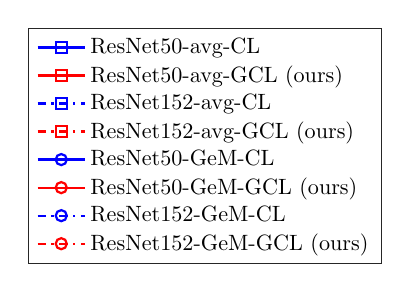
\begin{tikzpicture}[thick, scale=1, every node/.style={scale=.8}] 
    \begin{axis}[%
    hide axis,
    xmin=20,
    xmax=50,
    ymin=0,
    ymax=0.4,
    height=6cm, width=2cm,
    legend style={draw=white!15!black,legend cell align=left}
    ]
\addlegendimage{blue, mark size=2pt, thick , mark=square, style=solid,mark options=solid}
\addlegendentry{ResNet50-avg-CL};
\addlegendimage{red, mark size=2pt, thick , mark=square, style=solid,mark options=solid}
\addlegendentry{ResNet50-avg-GCL (ours)};
\addlegendimage{blue, mark size=2pt, thick , mark=square, style=dashdotted,mark options=solid}
\addlegendentry{ResNet152-avg-CL};
\addlegendimage{red, mark size=2pt, thick , mark=square, style=dashdotted,mark options=solid}
\addlegendentry{ResNet152-avg-GCL (ours)};
\addlegendimage{blue, mark size=2pt, thick , mark=o, style=solid,mark options=solid}
\addlegendentry{ResNet50-GeM-CL};
\addlegendimage{red, mark size=2pt, thick , mark=o, style=solid,mark options=solid}
\addlegendentry{ResNet50-GeM-GCL (ours)};
\addlegendimage{blue, mark size=2pt, thick , mark=o, style=dashdotted,mark options=solid}
\addlegendentry{ResNet152-GeM-CL};
\addlegendimage{red, mark size=2pt, thick , mark=o, style=dashdotted,mark options=solid}
\addlegendentry{ResNet152-GeM-GCL (ours)};
    \end{axis}
    \end{tikzpicture} 

\end{minipage}
}

   \caption{Comparison of the results achieved by methods trained with GCL and CL for (a) different distance thresholds and (b) different $\psi$ threshold values. GCL-based methods are plotted in red, while CL-based methods are shown in blue.}
       \label{fig:msls_psi_dist}

\end{figure*}


\revised{\subsection{Detailed results on RobotCar Seasons v2 and Extended CMU Seasons}

We provide results divided by type of environment for the Extended CMU Dataset and display them in Table~\ref{tab:cmu_detailed}. We observed that all models (ours and SoTA ones) tend to reach a higher performance on the urban images. This is logical, as they are all trained on datasets with images depicting mainly urban areas. 

We also provide detailed results for the RobotCar Seasons v2 dataset, organized by weather and illumination conditions, in Table~\ref{tab:robotcar_extended}. We observe that all methods obtain a higher successful localization rate on day conditions, but our methods tend to outperform the state-of-the-art on the night-time subsets. The MSLS train dataset includes images taken at night, but those are heavily underrepresented, so it is very interesting that GCL based models can localize images under these conditions.

}



















\revised{\subsection{Comparison to Thoma et al~\cite{thoma2020soft}}
In Table~\ref{tab:comparisonwiththoma}, we show the results that we obtained on the first version of the CMU dataset, and we compare our performance to the one achieved by the method presented in~\cite{thoma2020soft}. Our method is trained on the MSLS dataset, while the model of~\cite{thoma2020soft} is a NetVLAD model trained on the Oxford RobotCar dataset~\cite{Maddern2017}. We observe that our method generalizes as well as~\cite{thoma2020soft} to this unseen dataset with the same VGG backbone, and significantly better when using a bigger backbone like ResNeXt. It is worth noting that our method uses a simple pooling method (namely GeM~\cite{radenovic2018fine}), while~\cite{thoma2020soft} deploys a VLAD layer.}




\begin{figure*}[t]
\subfloat[heads]{
\centering
\includegraphics[width=.25\textwidth]{figures/appendix/7Scenes/headsprcurve.pdf}
}\hspace{-0.5cm}
\subfloat[stairs]{
\centering
\includegraphics[width=.25\textwidth]{figures/appendix/7Scenes/stairsprcurve.pdf}
}\hspace{-0.5cm}
\subfloat[pumpkin]{
\centering
\includegraphics[width=.25\textwidth]{figures/appendix/7Scenes/pumpkinprcurve.pdf}
}
\subfloat{
\centering
\includegraphics[width=.25\textwidth]{figures/appendix/7Scenes/legendprcurve.pdf}
}
\setcounter{subfigure}{3}
\hspace{-0.5cm}\subfloat[fire]{
\centering
\includegraphics[width=.25\textwidth]{figures/appendix/7Scenes/fireprcurve.pdf}
}\hspace{-0.5cm}
\subfloat[redkitchen]{
\centering
\includegraphics[width=.25\textwidth]{figures/appendix/7Scenes/redkitchenprcurve.pdf}
}\hspace{-0.5cm}
\subfloat[chess]{
\centering
\includegraphics[width=.25\textwidth]{figures/appendix/7Scenes/chessprcurve.pdf}
}\hspace{-0.5cm}
\subfloat[office]{
\centering
\includegraphics[width=.25\textwidth]{figures/appendix/7Scenes/officeprcurve.pdf}
}
 \caption{Precision-recall curves achieved on the 7Scenes dataset by ResNet18 and ResNet34 models trained using the Contrastive Loss function (CL, blue lines) and the proposed Generalized Contrastive loss (GCL, red lines) function.}
    \label{fig:7scenes_pr}
\end{figure*}






%%%% -----------------------------------------------------

% 

%%%% -----------------------------------------------------
\begin{table*}[t!]
\centering
\caption{Median translation and rotation errors (in cm and degrees, respectively) on the 7Scenes dataset using the descriptors computed using the models trained with the binary Contrastive Loss and the Generalized Contrastive Loss for retrieval and InLoc for localization.}
\label{tab:7scenes_loc}
\setlength\tabcolsep{2.5pt}

\begin{tabular*}{\textwidth}{@{}l@{\extracolsep{\fill}}llllllll@{}}
\toprule
\textbf{Model} & \textbf{heads}    & \textbf{stairs} & \textbf{pumpkin} & \textbf{fire} & \textbf{redkitchen} & \textbf{office} & \textbf{chess} & \textbf{Mean}  \\ \midrule
NetVLAD-DensePE & 2cm 1.16$\degree$ & 9cm 2.47$\degree$ & 5cm 1.55$\degree$ & 3cm 1.07$\degree$ &4cm 1.31$\degree$ & 3cm 1.05$\degree$ & 3cm 1.05$\degree$& 4.14cm 1.38$\degree$\\
ResNet34-CL   & 2.98cm 2.44$\degree$      & 36.03cm 4.28$\degree$   & 7.12cm 1.97$\degree$     & 5.87cm 2.39$\degree$  & 6.53cm 2.12$\degree$        & 5.62cm 1.85$\degree$    & 6.01cm 1.99$\degree$   & 10.02cm 2.43$\degree$ \\
ResNet34-GCL  & 2.53cm 2.3$\degree$ & 32.13cm 3.9$\degree$    & 6.4cm 1.95$\degree$      & 5.13cm 2.11$\degree$  & 5.38cm 2.0$\degree$         & 5.16cm 1.7$\degree$     & 5.66cm 1.93$\degree$   & 8.91cm 2.27$\degree$  \\ \bottomrule
\end{tabular*}
\end{table*}






\subsection{Performance for different ground truths}

We performed an evaluation of the performance that the models that we train achieved when varying the ground truth threshold, i.e. when applying different cut values on the criteria that define two images as similar or not. We report results on the MSLS validation dataset.

First, we consider the distance, computed using the GPS coordinates associated to image pairs, between the location from where the images were taken and define a threshold on this value. For instance, we consider as similar all the image pairs that were taken from places with a distance lower than $D$, and vary $D$ between $5$ meters to $50$ meters. We report the result in  Fig.~\ref{fig:msls_dist}. An image is considered as correctly identified if at least one of the top-5 retrieved images is at a distance smaller than the considered threshold.

Furthermore, we consider the defined graded similarity $\psi$ and threshold it with values between $0$ and $0.9$. An image is considered as correctly identified if at least one of the top-5 retrieved images is labeled with a similarity greater than the considered threshold. We report the results in Fig.~\ref{fig:msls_psi_dist}.

In both cases, the models trained using the GCL function are more robust than those trained using the CL function to variations of the criteria and values used to establish the ground truth similarity between image pairs.


\subsection{Extra results on 7Scenes}


\textbf{Precision-recall curve.} We report the precision recall curves that we obtained on the 7Scenes dataset in Fig.~\ref{fig:7scenes_pr}. The models trained with the GCL function (red lines) consistently outperform their counterpart trained with the CL function (blue lines),  when they deploy both the ResNet18 and ResNet34 backbones. The results are consistent for all the sub-sets of the 7Scenes dataset. The case of the \emph{chess} scene is particularly interesting, for which the ResNet34-GCL model achieved near-perfect performance.

\revised{
\textbf{Localization. }
We tested the impact that a model trained with the GCL function and graded similarity has on the performance of a camera localization pipeline. We compared it to the case when the same model trained with the original binary Contrastive Loss function is used for the image retrieval task, and report the localization error that we obtained in Table~\ref{tab:7scenes_loc}. This experiment is meant only to demonstrate that the general expectation of better retrieval results contribute to better localization' is satisfied by the improved retrieval results achieved using the proposed GCL. For this experiment, we employed the InLoc algorithm~\cite{taira2018inloc}, using our learned representations with the ResNet34 backbone for the retrieval step. The images retrieved using the representation learned with GCL consistently led to an improvement of the localization accuracy w.r.t. the case in which the CL function is used. The enhanced performance of the retrieval task has a positive effect on the precision of localization algorithms. We also report the results of the original InLoc pipeline, based on and optimized to work with a NetVLAD backbone. While the GCL function contributes indirectly to better localization w.r.t. its binary CL counterpart, it requires more work to be effectively embedded in a localization pipeline.





}

\begin{comment}

\subsection{Performance for smaller input images}
\begin{table}[t]
\centering
\caption{Additional results on the MSLS test set for images of input size 224x224.}
\label{tab:msls-224}
\setlength\tabcolsep{4pt}
\begin{tabular}{@{}lllllcc@{}}
\toprule
\textbf{\textbf{Backbone}} &
  \textbf{\textbf{Input size}} &
  \textbf{\textbf{Pooling}} &
  \textbf{\textbf{Loss}} &
  \textbf{\textbf{R@1}} &
  \textbf{\textbf{R@5}} &
  \textbf{\textbf{R@10}} \\ \midrule
\multirow{10}{*}{ResNet50} & \multirow{2}{*}{224x224} & \multirow{2}{*}{avg} & CL       & 15.6 & 27.8                     & 34.9                     \\
         &                          &                      & GCL      & 26.1 & 42                       & 48.5                     \\ \cmidrule(l){2-7} 
         & \multirow{2}{*}{480x640} & \multirow{2}{*}{avg} & CL       & 24.9 & 39.0                     & 44.6                     \\
         &                          &                      & GCL      & 35.8 & 52.0                     & 59.0                     \\ \cmidrule(l){2-7} 
 &
  \multirow{4}{*}{224x224} &
  \multirow{4}{*}{GeM} &
  TL~\cite{warburg2020bayesian} &
  37.2 &
  52.2 &
  58.2 \\
         &                          &                      & Bayes TL~\cite{warburg2020bayesian} & 36.6 & 51.3 & 57.4 \\
         &                          &                      & CL       & 17.3 & 31.8                     & 37.9                     \\
         &                          &                      & GCL      & 28.7 & 44.1                     & 50.3                     \\ \cmidrule(l){2-7} 
         & \multirow{2}{*}{480x640} & \multirow{2}{*}{GeM} & CL       & 29.7 & 44.0                     & 50.7                     \\
         &                          &                      & GCL      & 43.3 & 59.1                     & 65.0                     \\ \midrule
\multirow{8}{*}{ResNet152} &
  \multirow{2}{*}{224x224} &
  \multirow{2}{*}{avg} &
  CL &
  18.9 &
  32.2 &
  38.2 \\
         &                          &                      & GCL      & 30.8 & 44.9                     & 52.8                     \\ \cmidrule(l){2-7} 
         & \multirow{2}{*}{480x640} & \multirow{2}{*}{avg} & CL       & 29.7 & 44.2                     & 51.3                     \\
         &                          &                      & GCL      & 43.5 & 59.2                     & 65.2                     \\ \cmidrule(l){2-7} 
         & \multirow{2}{*}{224x224} & \multirow{2}{*}{GeM} & CL       & 22.5 & 37.6                     & 43.8                     \\
         &                          &                      & GCL      & 32.1 & 47.3                     & 54.3                     \\ \cmidrule(l){2-7} 
         & \multirow{2}{*}{480x640} & \multirow{2}{*}{GeM} & CL       & 34.1 & 50.8                     & 56.8                     \\
         &                          &                      & GCL      & \textbf{45.7} & \textbf{62.3}            & \textbf{67.9}            \\ \bottomrule
\end{tabular}
\end{table}

Complex models are often trained using lower resolution images, in order to better use the hardware resources used for the training process within their physical limitations. We report the results that we achieved on the MSLS test set by training models with the CL and GCL function on images of resolution $224\times224$. We achieved lower results than other methods that use the triplet or Bayes triplet loss function. Although the GCL function contributes to a consistent improvement of performance w.r.t. when the CL function is used, we attribute the decrease of performance of our methods to the less and lower resolution information  that we can exploit to learn robust representation for image similarity. However, as the memory requirements of our method are much lower than those of other more complicate methods, and we do not need to perform a memory-intensive mining process to select training pairs, we can train our methods using bigger images and use large batches of images (up to 512 images on an Nvidia V100 GPU).

\end{comment}
